\documentclass[x11names, svgnames, rgb]{beamer}

\usetheme{Madrid}
% \usecolortheme{beaver}

% you can only do these with very special types of pdf viewers
% \usepackage{animate}
% \animategraphics[loop,controls,width=\linewidth]{10}{imgs/serialPartition-}{0}{129}
% \usepackage{xmpmulti}
\usepackage{algpseudocode}

\usepackage{mathtools}
\newcommand{\defeq}{\vcentcolon=}
\DeclarePairedDelimiter{\paren}{(}{)}

\newcommand{\dec}{\operatorname{dec}}
\newcommand{\poly}{\operatorname{poly}}
\newcommand{\polylog}{\operatorname{polylog}}
\newcommand{\github}{\url{github.com/awestover/Parallel-Partition}}
\newcommand{\defn}[1]       {{\textit{\textbf{\boldmath #1}}}}
\newcommand{\paragraph}[1]{\vspace{0.09in}\noindent{\bf \boldmath #1.}} 
\usepackage{amsmath}
\def\E{\operatorname{\mathbb{E}}}
\usepackage{amssymb}
\usepackage{amsthm}

\newtheorem{proposition}{Proposition}
\newtheorem{defin}{Definition}

\usepackage{hyperref}


\title{Cache-Efficient Parallel Partition Algorithms}
\author{Alek Westover}
\institute{MIT PRIMES}
\date{October 20, 2019}

\begin{document}
 
\frame{\titlepage}

\begin{frame}[t]{Partition}
	\begin{defin}[Partitioned Array]
		$A[i]$ predecessor, $A[j]$ successor $\implies i < j$
	\end{defin}	
	\begin{defin}[Array partitioned relative to pivot value $p$]
		$A[i] \le p, A[j] > p \implies i < j$
	\end{defin}	
	\begin{figure}
		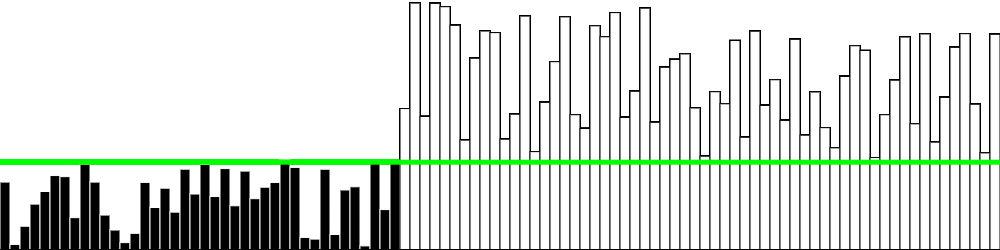
\includegraphics[width=\linewidth]{imgs/partitionedArray.png}
		\caption{Black: Predecessor, White: Successor, Green: Pivot Value}
	\end{figure}
\end{frame}

\begin{frame}[t]{Parallel Algorithm}
	\begin{figure}
		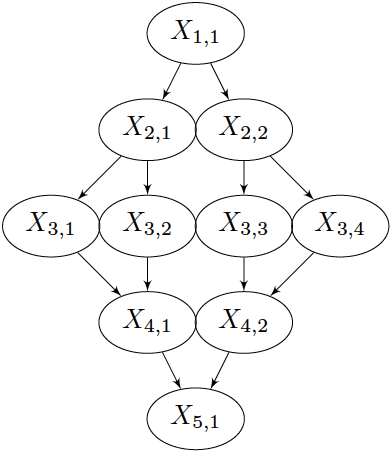
\includegraphics[width=0.5\linewidth]{imgs/DAG.png}
	\end{figure}
\end{frame}

\begin{frame}[t]{Work and Span}

\begin{defin}[$T_p$]
	Running time on $p$ processors. Note: $T_p \ge T_\infty, T_p \ge \frac{T_1}{p}$.
\end{defin}	
\begin{defin}[Work]
	Running time on a single processor. $T_1 = \sum_i W_i$.
\end{defin}	
\begin{defin}[Span]
	Running time on infinitely many processors. $T_\infty = \sum_i 1$.
\end{defin}	
\begin{theorem}[Brent's Theorem]
	$$T_p = \sum_i \Big\lceil \frac{W_i}{p} \Big\rceil \le \sum_i \Big( \frac{W_i}{p}+1 \Big) = \frac{T_1}{p}+T_\infty.$$	
\end{theorem}
\end{frame}

\begin{frame}[t]{Serial Partition}  %% See if you can get a decent picture replacement for this...
  % \transduration<0-10>{0}
	% \multiinclude[<+->][format=png, graphics={width=\textwidth}]{imgs/serialPartition-}
	\begin{algorithmic}
		\While{$\text{low} < \text{high}$} 
	\While{$A[\text{low}] \leq \text{pivotValue}$}
			\State $\text{low} \gets \text{low}+1$
		\EndWhile
		\While{$A[\text{high}] > \text{pivotValue}$}
		\State $\text{high} \gets \text{high}-1$
		\EndWhile
		\State Swap $A[\text{low}]$ with $A[\text{high}]$
	\EndWhile
	\If{$A[\text{low}] \leq \text{pivotValue}$}
	\State $\text{low} \gets \text{low}+1$
	\EndIf
\end{algorithmic}

\end{frame}

\begin{frame}[t]{Randomized Algorithms}
	\begin{defin}[With high probability in $n$]
		Probability of success is 
		$$1-\frac{1}{n^c}$$
		for $c$ of our choice. i.e. the probability can be made arbitrarily close to $1$.
	\end{defin}
\end{frame}

\begin{frame}[t]{Memory Bandwidth Bound}
	\begin{defin}[Cache miss]
		A cache miss occurs when the algorithm must load a cache-line not stored in cache into cache.
	\end{defin}	
	\begin{itemize}
		\item In-place is desirable.
		\item Kuszmaul developed an in-place version of parallel partition.
		\item His in-place version outperformed the out-of-place standard algorithm.
		\item But was outperformed in practice by a more cache efficient, higher span algorithm.
		\item Experiments show the source of the problem: Memory bandwidth bound, i.e. incurring too many cache misses.
		\item Note that both temporal and spatial cache efficiency are important.
	\end{itemize}
\end{frame}

\begin{frame}[t]{Strided Algorithm cite{FrancisPa92, Frias08} Description}
	Partition $A$ into chunks $C_1,C_2,\ldots C_n/gb$ each consisting of $g$ cache lines of size $b$. Let $P_i$ be the union of the $i$-th cache-line from each chunk $C_j$.
	\begin{figure}
		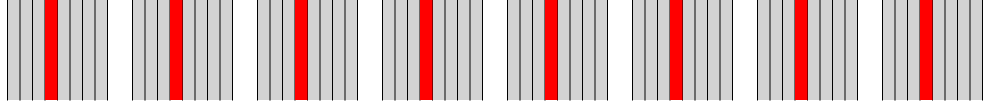
\includegraphics[width=\linewidth]{imgs/stridedAlgHighlighted.png}
	\end{figure}
	\begin{defin}[Partially Partitioned Array]
		$\exists u, l $ such that $$i < u \implies A[i] \text{ is predecessor }, i \ge l \implies A[i] \text{ is successor }$$
	\end{defin}
	\begin{itemize}
		\item Perform serial partitions on all $P_i$ in parallel.
		\item Let $v_i$ be the position in $A$ of the first successor in $P_i$. Perform a serial partition on $A[\min_i v_i], \ldots, A[\max_i v_i -1]$.
	\end{itemize}
\end{frame}

\begin{frame}[t]{Strided Algorithm Analysis}
	\begin{itemize}
		\item Partial partiton step: work $O(n)$, span $\Theta(n/g)$.
		\item Serial cleanup step: span $\Theta(v_\text{max}-v_\text{min})$, which is $O(n)$ in general.
		\item If the number of predecessors in each $P_i$ is similar, $v_\text{max}-v_\text{min}$ can be small.
		\item In particular, if $b\in \polylog(n)$, and the array values are selected independently at random from some distribution, and $g$ is chosen to optimize span ($g=n^{1/3}$), then with high probability in $n$, $$v_\text{max}-v_\text{min} < \tilde{O}(n^{2/3}),$$ the span is $$\tilde{O}(n^{2/3}),$$ and the number of cache misses is fewer than $$\frac{n}{b}+\frac{\tilde{O}(n^{2/3})}{b}.$$
	\end{itemize}
\end{frame}


\begin{frame}[t]{Smoothed Striding Algorithm Description}
	Let $X[1],\ldots, X[s]$ be chosen uniformly at random from $\{1,\ldots, g\}$. Let $U_i$ be the union of the $(X[j]+i)\mod g$-th cache-line from each chunk $C_j$.
	\begin{figure}
		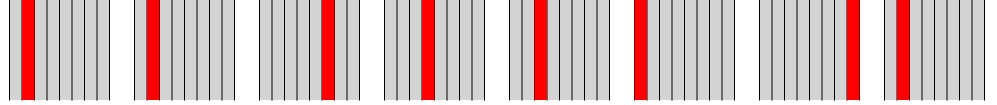
\includegraphics[width=\linewidth]{imgs/smoothedStridingAlgHighlighted.png}
	\end{figure}
	\begin{itemize}
		\item Perform serial partitions on all $U_i$ in parallel.
		\item The array is partially now partitioned with $A[i]$ a predecessor for all $i < v_{\text{min}}$ and $A[i]$ a successor for all $i \ge v_{\text{max}}$.
	\end{itemize}
	Note that we will make $s = \frac{n}{gb} < \polylog(n)$ so the algorithm remains in-place.
\end{frame}


\begin{frame}[t]{Partial Partition Step Analysis}
\begin{proposition}
  %% The 1/2's are necessary for the final line of the proof to easily go through.
  Let $\epsilon \in (0, 1/2)$ and $\delta \in (0, 1/2)$ such that
  $\epsilon \ge \frac{1}{\poly(n)}$ and $\delta \ge
  \frac{1}{\polylog(n)}$. Suppose $s > \frac{\ln
    (n/\epsilon)}{\delta^2}$. Finally, suppose that each processor has
  a cache of size at least $s + c$ for a sufficiently large constant
  $c$.

  Then the Partial-Partition Algorithm achieves work $O(n)$; achieves
  span $O\paren*{b \cdot s}$; incurs $\frac{s+n}{b} + O(1)$ cache
  misses; and guarantees with probability $1 - \epsilon$ that
  $$v_{\text{max}}-v_{\text{min}} < 4 n \delta.$$
\end{proposition}

\end{frame}

\begin{frame}[t]{From Partial Partition to Full Partition}
	\emph{Partial Partition Step:}
	\begin{itemize}
		\item Use $\epsilon = 1/n^c$ for $c$ of our choice (i.e. with high probability).
		\item Choice of $\delta$ results in tradeoff between cache misses and span.
	\end{itemize}
	\emph{Recursive strategies:}
	\begin{itemize}
		\item \defn{Hybrid Smoothed Striding Algorithm}: Use algorithm with span $O(\log n \log \log n)$. Note: recursive algorithm's cache behavior doesn't affect overall cache behavior because subarray is small. This algorithm can be tuned to give optimal span and cache misses.
		\item \defn{Recursive Smoothed Striding Algorithm}: Use the Partial Partition step recursively to solve subproblems. Recursive applications of the Partial Partition step use the same $\epsilon$ the top-level (to guarantee success with high probability in $n$), and use $\delta \in \Theta(1)$ such that the problem size is reduced by half at each step. This algorithm has slightly worse span, but is very simple to implement.
	\end{itemize}
\end{frame}



\begin{frame}[t]{Hybrid Algorithm Analysis - General Theorem}
\begin{theorem}
	The Hybrid Smoothed Striding Algorithm algorithm using parameter $\delta\in(0,1/2)$ satisfying $\delta \ge 1/\polylog(n)$: has work $O(n)$; achieves span
        $$O\paren*{\log n \log\log n +\frac{b\log n}{\delta^2}},$$
with high probability in $n$; and incurs fewer than 
$$(n+O(n\delta))/b$$
cache misses with high probability in $n$.
\end{theorem}
\end{frame}

\begin{frame}[t]{Hybrid Algorithm Analysis - Corollary for specific parameter settings}
An interesting corollary of the above theorem concerns what happens when $b$ is small (e.g., constant) and we choose $\delta$ to optimize span. 
\begin{corollary}
Suppose $b \le o(\log \log n)$. Then the Cache-Efficient Full-Partition Algorithm algorithm using $\delta = \Theta\big(\sqrt{b/\log\log n}\big)$, achieves work $O(n)$, and with high probability in $n$, achieves span $O(\log n \log\log n)$ and incurs fewer than $(n+o(n))/b$ cache misses.
\end{corollary}
\end{frame}


\begin{frame}[t]{Recursive Algorithm Analysis - General Theorem}
	\begin{theorem}
	With high probability in $n$, the Recursive Smoothed Striding
        algorithm using parameter $\delta \in(0,1/2)$ satisfying
        $\delta \ge 1 / \polylog(n)$: achieves work $O(n)$, attains span
	$$O\left(b\left(\log^2 n + \frac{\log n}{\delta^2}\right)\right),$$
	and incurs $(n+O(n \delta))/b$ cache misses. 
	\end{theorem}
\end{frame}

\begin{frame}[t]{Recursive Algorithm Analysis - Corollary for specific parameter settings}
A particularly natural parameter setting for the Recursive algorithm occurs at $\delta = 1 / \sqrt{\log n}$.
\begin{corollary}
	With high probability in $n$, the Recursive Smoothed Striding Algorithm using parameter $\delta=1/\sqrt{\log n}$:
  achieves work $O(n)$, attains span $O(b\log^2 n)$, and incurs $n/b \cdot (1 + O(1 / \sqrt{\log n}))$ cache misses. 
\end{corollary}
\end{frame}

\begin{frame}[t]{Experiments}
	\begin{itemize}
		\item Strided Algorithm vs Smoothed Striding algorithm
		\item Cache misses 
	\end{itemize}
\end{frame}

\begin{frame}[t]{Acknowledgments}
I would like to thank
\begin{itemize}
	\item {The MIT PRIMES program}
	\item {William Kuszmaul, my PRIMES mentor}
	\item {My parents}
\end{itemize}
\end{frame}

\begin{frame}[t]{References}
	 \bibliographystyle{ACM-Reference-Format}
	\bibliography{paper}
\end{frame}

\end{document}
